\documentclass[12pt]{article}
\usepackage[a4paper, margin=1in]{geometry}
\usepackage{graphicx}
\usepackage{titlesec}
\usepackage{longtable}
\usepackage{tabularx}
\usepackage{booktabs}
\usepackage{setspace}
\usepackage{hyperref}
\usepackage{array}
\usepackage{caption}
\usepackage{multirow}
\usepackage{listings}
\usepackage{xcolor}
\usepackage{subfig}
\usepackage{float}
\usepackage{amsmath}   % For improved math support
\usepackage{amssymb}   % Additional math symbols
\usepackage{enumitem}  % Customizable lists
\usepackage{fancyhdr}  % Custom headers and footers
\usepackage{siunitx}   % SI unit formatting
\usepackage{bm}        % Bold math symbols

\lstset{
    language=C,
    basicstyle=\ttfamily\footnotesize,
    keywordstyle=\color{blue},
    commentstyle=\color{gray},
    stringstyle=\color{red},
    breaklines=true,
    numbers=left,
    numberstyle=\tiny\color{gray},
    frame=single
}

\onehalfspacing
\setcounter{secnumdepth}{3}
\setcounter{tocdepth}{2}

\begin{document}

\begin{titlepage}
    \begin{center}
        
\includegraphics[width=0.3\textwidth]{AURAK Logo.jpg}\\[1cm]
        \textbf{\LARGE American University of Ras Al Khaimah}\\[2cm]
        \textbf{\Huge Microprocessors Lab}\\[0.5cm]
        \textbf{\Large CENG316}\\[1.5cm]
        \textbf{\large Section: 1}\\[0.2cm]
        \textbf{\large Instructor: Engr. Umar Adeel}\\[2cm]
        \textbf{\Large Lab 3 -- Keypad Scanning in C}\\[2cm]
        \textbf{\large Abin Raj Devarajan\hspace{1cm}2022005464}\\[2cm]
        \textbf{\large Date of the lab: 09--02--2025}
    \end{center}
\end{titlepage}

\newpage
\tableofcontents
\newpage

\section{Objective}
\begin{itemize}
    \item Understand the process of scanning a keypad matrix using GPIO.
    \item Implement an efficient keypad scanning algorithm using software debouncing.
    \item Display pressed keys dynamically on an LCD, ensuring smooth scrolling.
    \item Handle multiple keypress scenarios with proper debounce techniques.
\end{itemize}

\section{Equipment Used}
\begin{itemize}
    \item STM32L476G-DISCO board
    \item 4x4 matrix keypad
    \item LCD display
    \item Breadboard and jumper wires
    \item 2.2k Ohm pull-up resistors
    \item KEIL tool by ARM
\end{itemize}


\section{Pre-Lab}
\addcontentsline{toc}{section}{Pre-Lab}
\label{sec:prelab}

\subsection{Part A – Textbook Readings}
Before beginning the lab, students are required to review the following section from the textbook:
\begin{itemize}
    \item \textbf{Chapter 14.9:} Keypad scanning
\end{itemize}

\subsection{Part B – Pre-Lab Assignment}
In this lab, we will interface with a keypad using the STM32 microcontroller. The keypad and necessary components such as a breadboard and wires will be provided. Due to the board design, it is recommended to use two breadboards for better connectivity.

We will configure specific pins on \textbf{GPIOA} as inputs and \textbf{GPIOE} as outputs to facilitate the keypad scanning process.

\subsubsection{ Configure Port A (Inputs)}
We will set GPIOA pins 1, 2, 3, and 5 as digital inputs. These pins are also used by the joystick but will be reassigned for external connections in this experiment.

The configuration is achieved by setting the GPIOA MODER register, where:
\begin{itemize}
    \item \texttt{00} (binary) represents digital input mode.
\end{itemize}

\bigskip

\noindent\textbf{Register Layout for MODER (Port A)}
\begin{table}[H]
    \centering
    \scriptsize % Set a smaller font size for the table
    \renewcommand{\arraystretch}{1.2} % Adjust row height
    \setlength{\tabcolsep}{1.5pt} % Adjust column spacing
    \begin{tabular}{|c|*{32}{c|}}
        \hline
        \textbf{Register} 
        & \textbf{31} & \textbf{30} & \textbf{29} & \textbf{28} 
        & \textbf{27} & \textbf{26} & \textbf{25} & \textbf{24} 
        & \textbf{23} & \textbf{22} & \textbf{21} & \textbf{20} 
        & \textbf{19} & \textbf{18} & \textbf{17} & \textbf{16}
        & \textbf{15} & \textbf{14} & \textbf{13} & \textbf{12} 
        & \textbf{11} & \textbf{10} & \textbf{9} & \textbf{8} 
        & \textbf{7} & \textbf{6} & \textbf{5} & \textbf{4} 
        & \textbf{3} & \textbf{2} & \textbf{1} & \textbf{0} \\ \hline
        
        \textbf{MODER} 
        & \multicolumn{2}{|c|}{\rotatebox{90}{MODER15}} & \multicolumn{2}{|c|}{\rotatebox{90}{MODER14}} 
        & \multicolumn{2}{|c|}{\rotatebox{90}{MODER13}} & \multicolumn{2}{|c|}{\rotatebox{90}{MODER12}} 
        & \multicolumn{2}{|c|}{\rotatebox{90}{MODER11}} & \multicolumn{2}{|c|}{\rotatebox{90}{MODER10}} 
        & \multicolumn{2}{|c|}{\rotatebox{90}{MODER9}} & \multicolumn{2}{|c|}{\rotatebox{90}{MODER8}}
        & \multicolumn{2}{|c|}{\rotatebox{90}{MODER7}} & \multicolumn{2}{|c|}{\rotatebox{90}{MODER6}}
        & \multicolumn{2}{|c|}{\rotatebox{90}{MODER5}} & \multicolumn{2}{|c|}{\rotatebox{90}{MODER4}}
        & \multicolumn{2}{|c|}{\rotatebox{90}{MODER3}} & \multicolumn{2}{|c|}{\rotatebox{90}{MODER2}}
        & \multicolumn{2}{|c|}{\rotatebox{90}{MODER1}} & \multicolumn{2}{|c|}{\rotatebox{90}{MODER0}}\\ \hline

        \textbf{Mask}
        & 0 & 0 & 0 & 0 
        & 0 & 0 & 0 & 0 
        & 0 & 0 & 0 & 0 
        & 0 & 0 & 0 & 0
        & 0 & 0 & 0 & 0
        & 0 & 0 & 0 & 0
        & 0 & 0 & 0 & 0
        & 0 & 0 & 0 & 0 \\ \hline
       
        \textbf{Value} 
        & 0 & 0 & 0 & 0 
        & 0 & 0 & 0 & 0 
        & 0 & 0 & 0 & 0
        & 0 & 0 & 0 & 0
        & 0 & 0 & 0 & 0
        & 0 & 0 & 0 & 0
        & 0 & 0 & 0 & 0
        & 0 & 0 & 0 & 0 \\ \hline
        
    \end{tabular}
    \caption{Mask in hex: 0x00000000 | Value in hex: 0x00000000}
    \label{tab:moder_configuration1}
\end{table}

\subsubsection{Configure Port E (Outputs)}
We will set GPIOE pins 10, 11, 12, and 13 as digital outputs to drive the keypad columns.

The configuration is achieved by modifying the GPIOE MODER register, where:
\begin{itemize}
    \item \texttt{01} (binary) represents digital output mode.
\end{itemize}

\bigskip

\noindent\textbf{Register Layout for MODER (Port E)}
\noindent\textbf{Register Layout for MODER (Port A)}
\begin{table}[H]
    \centering
    \scriptsize % Set a smaller font size for the table
    \renewcommand{\arraystretch}{1.2} % Adjust row height
    \setlength{\tabcolsep}{1.5pt} % Adjust column spacing
    \begin{tabular}{|c|*{32}{c|}}
        \hline
        \textbf{Register} 
        & \textbf{31} & \textbf{30} & \textbf{29} & \textbf{28} 
        & \textbf{27} & \textbf{26} & \textbf{25} & \textbf{24} 
        & \textbf{23} & \textbf{22} & \textbf{21} & \textbf{20} 
        & \textbf{19} & \textbf{18} & \textbf{17} & \textbf{16}
        & \textbf{15} & \textbf{14} & \textbf{13} & \textbf{12} 
        & \textbf{11} & \textbf{10} & \textbf{9} & \textbf{8} 
        & \textbf{7} & \textbf{6} & \textbf{5} & \textbf{4} 
        & \textbf{3} & \textbf{2} & \textbf{1} & \textbf{0} \\ \hline
        
        \textbf{MODER} 
        & \multicolumn{2}{|c|}{\rotatebox{90}{MODER15}} & \multicolumn{2}{|c|}{\rotatebox{90}{MODER14}} 
        & \multicolumn{2}{|c|}{\rotatebox{90}{MODER13}} & \multicolumn{2}{|c|}{\rotatebox{90}{MODER12}} 
        & \multicolumn{2}{|c|}{\rotatebox{90}{MODER11}} & \multicolumn{2}{|c|}{\rotatebox{90}{MODER10}} 
        & \multicolumn{2}{|c|}{\rotatebox{90}{MODER9}} & \multicolumn{2}{|c|}{\rotatebox{90}{MODER8}}
        & \multicolumn{2}{|c|}{\rotatebox{90}{MODER7}} & \multicolumn{2}{|c|}{\rotatebox{90}{MODER6}}
        & \multicolumn{2}{|c|}{\rotatebox{90}{MODER5}} & \multicolumn{2}{|c|}{\rotatebox{90}{MODER4}}
        & \multicolumn{2}{|c|}{\rotatebox{90}{MODER3}} & \multicolumn{2}{|c|}{\rotatebox{90}{MODER2}}
        & \multicolumn{2}{|c|}{\rotatebox{90}{MODER1}} & \multicolumn{2}{|c|}{\rotatebox{90}{MODER0}}\\ \hline

        \textbf{Mask}
        & 0 & 0 & 0 & 0 
        & 0 & 0 & 0 & 1 
        & 0 & 1 & 0 & 1 
        & 0 & 1 & 0 & 0
        & 0 & 0 & 0 & 0
        & 0 & 0 & 0 & 0
        & 0 & 0 & 0 & 0
        & 0 & 0 & 0 & 0 \\ \hline
       
        \textbf{Value} 
        & 0 & 0 & 0 & 0 
        & 0 & 0 & 1 & 1 
        & 1 & 1 & 1 & 1
        & 1 & 1 & 0 & 0
        & 0 & 0 & 0 & 0
        & 0 & 0 & 0 & 0
        & 0 & 0 & 0 & 0
        & 0 & 0 & 0 & 0 \\ \hline
        
    \end{tabular}
    \caption{Mask in hex: 0x00000000 | Value in hex: 0x00000000}
    \label{tab:moder_configuration1}
\end{table}
\bigskip

\section{Lab Procedure}
\textbf{Goal: }  The end goal of this lab is to be able to push buttons on the keypad, and have the values displayed on the
 LCD. The display should show the last 6 buttons pressed, and they should scroll off the screen to the left
 (similar to how a calculator or a telephone would enter the numbers). Software debouncing should be used
 to make sure no double-presses accidentally happen

\subsection{Part A – Connecting the Keypad}
\begin{enumerate}
    \item Connect the keypad to the STM32L4 GPIO pins:
    \begin{itemize}
        \item GPIOE (Pins 10, 11, 12, 13) for \textbf{row scanning}.
        \item GPIOA (Pins 1, 2, 3, 5) for \textbf{column scanning}.
    \end{itemize}
    \item Use external 2.2k ohm pull-up resistors on the column lines.
    \item Verify wiring using Figures 1 and 2 from the lab manual.
\end{enumerate}

\begin{figure}[h!]
    \centering
    \begin{minipage}{0.45\textwidth}
        \centering
    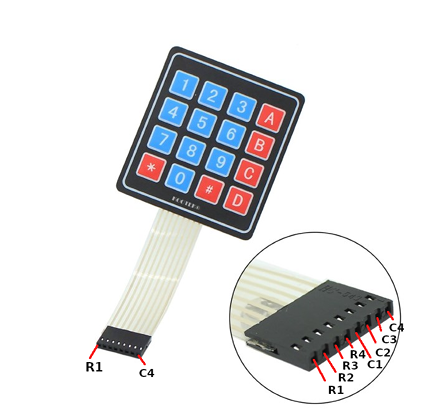
\includegraphics[width=\textwidth]{Screenshot 2025-02-11 224311.png}
    \caption{Keypad}\end{minipage}
    \hfill
    \begin{minipage}{0.45\textwidth}
        \centering
    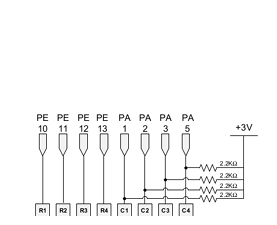
\includegraphics[width=\textwidth]{Screenshot 2025-02-11 224319.png}
    \caption{Row and Column code}
    \end{minipage}
\end{figure}


\subsection{Part B – Writing the Keypad Scanning Code}
\begin{enumerate}
    \item Modify \texttt{main.c} and add a function \texttt{Keypad\_Pin\_Init()} to configure GPIO.
    \item Implement the \texttt{keypad\_scan()} function to:
    \begin{itemize}
        \item Write `0b0000` to the rows.
        \item Read column values.
        \item Print scanned values to the LCD.
    \end{itemize}
    \item Implement row-wise scanning and column detection.
    \item Use a lookup table to map row-column combinations to keypad values.
\end{enumerate}

\subsection{Part C – Displaying Keypresses on the LCD}
\begin{enumerate}
    \item Implement a 6-character keypress buffer.
    \item Shift all stored keypresses one position left before adding a new key.
    \item Implement software debouncing to avoid repeated key registrations.
\end{enumerate}

\begin{figure}[h!]
    \centering
    \begin{minipage}{0.45\textwidth}
    \centering
    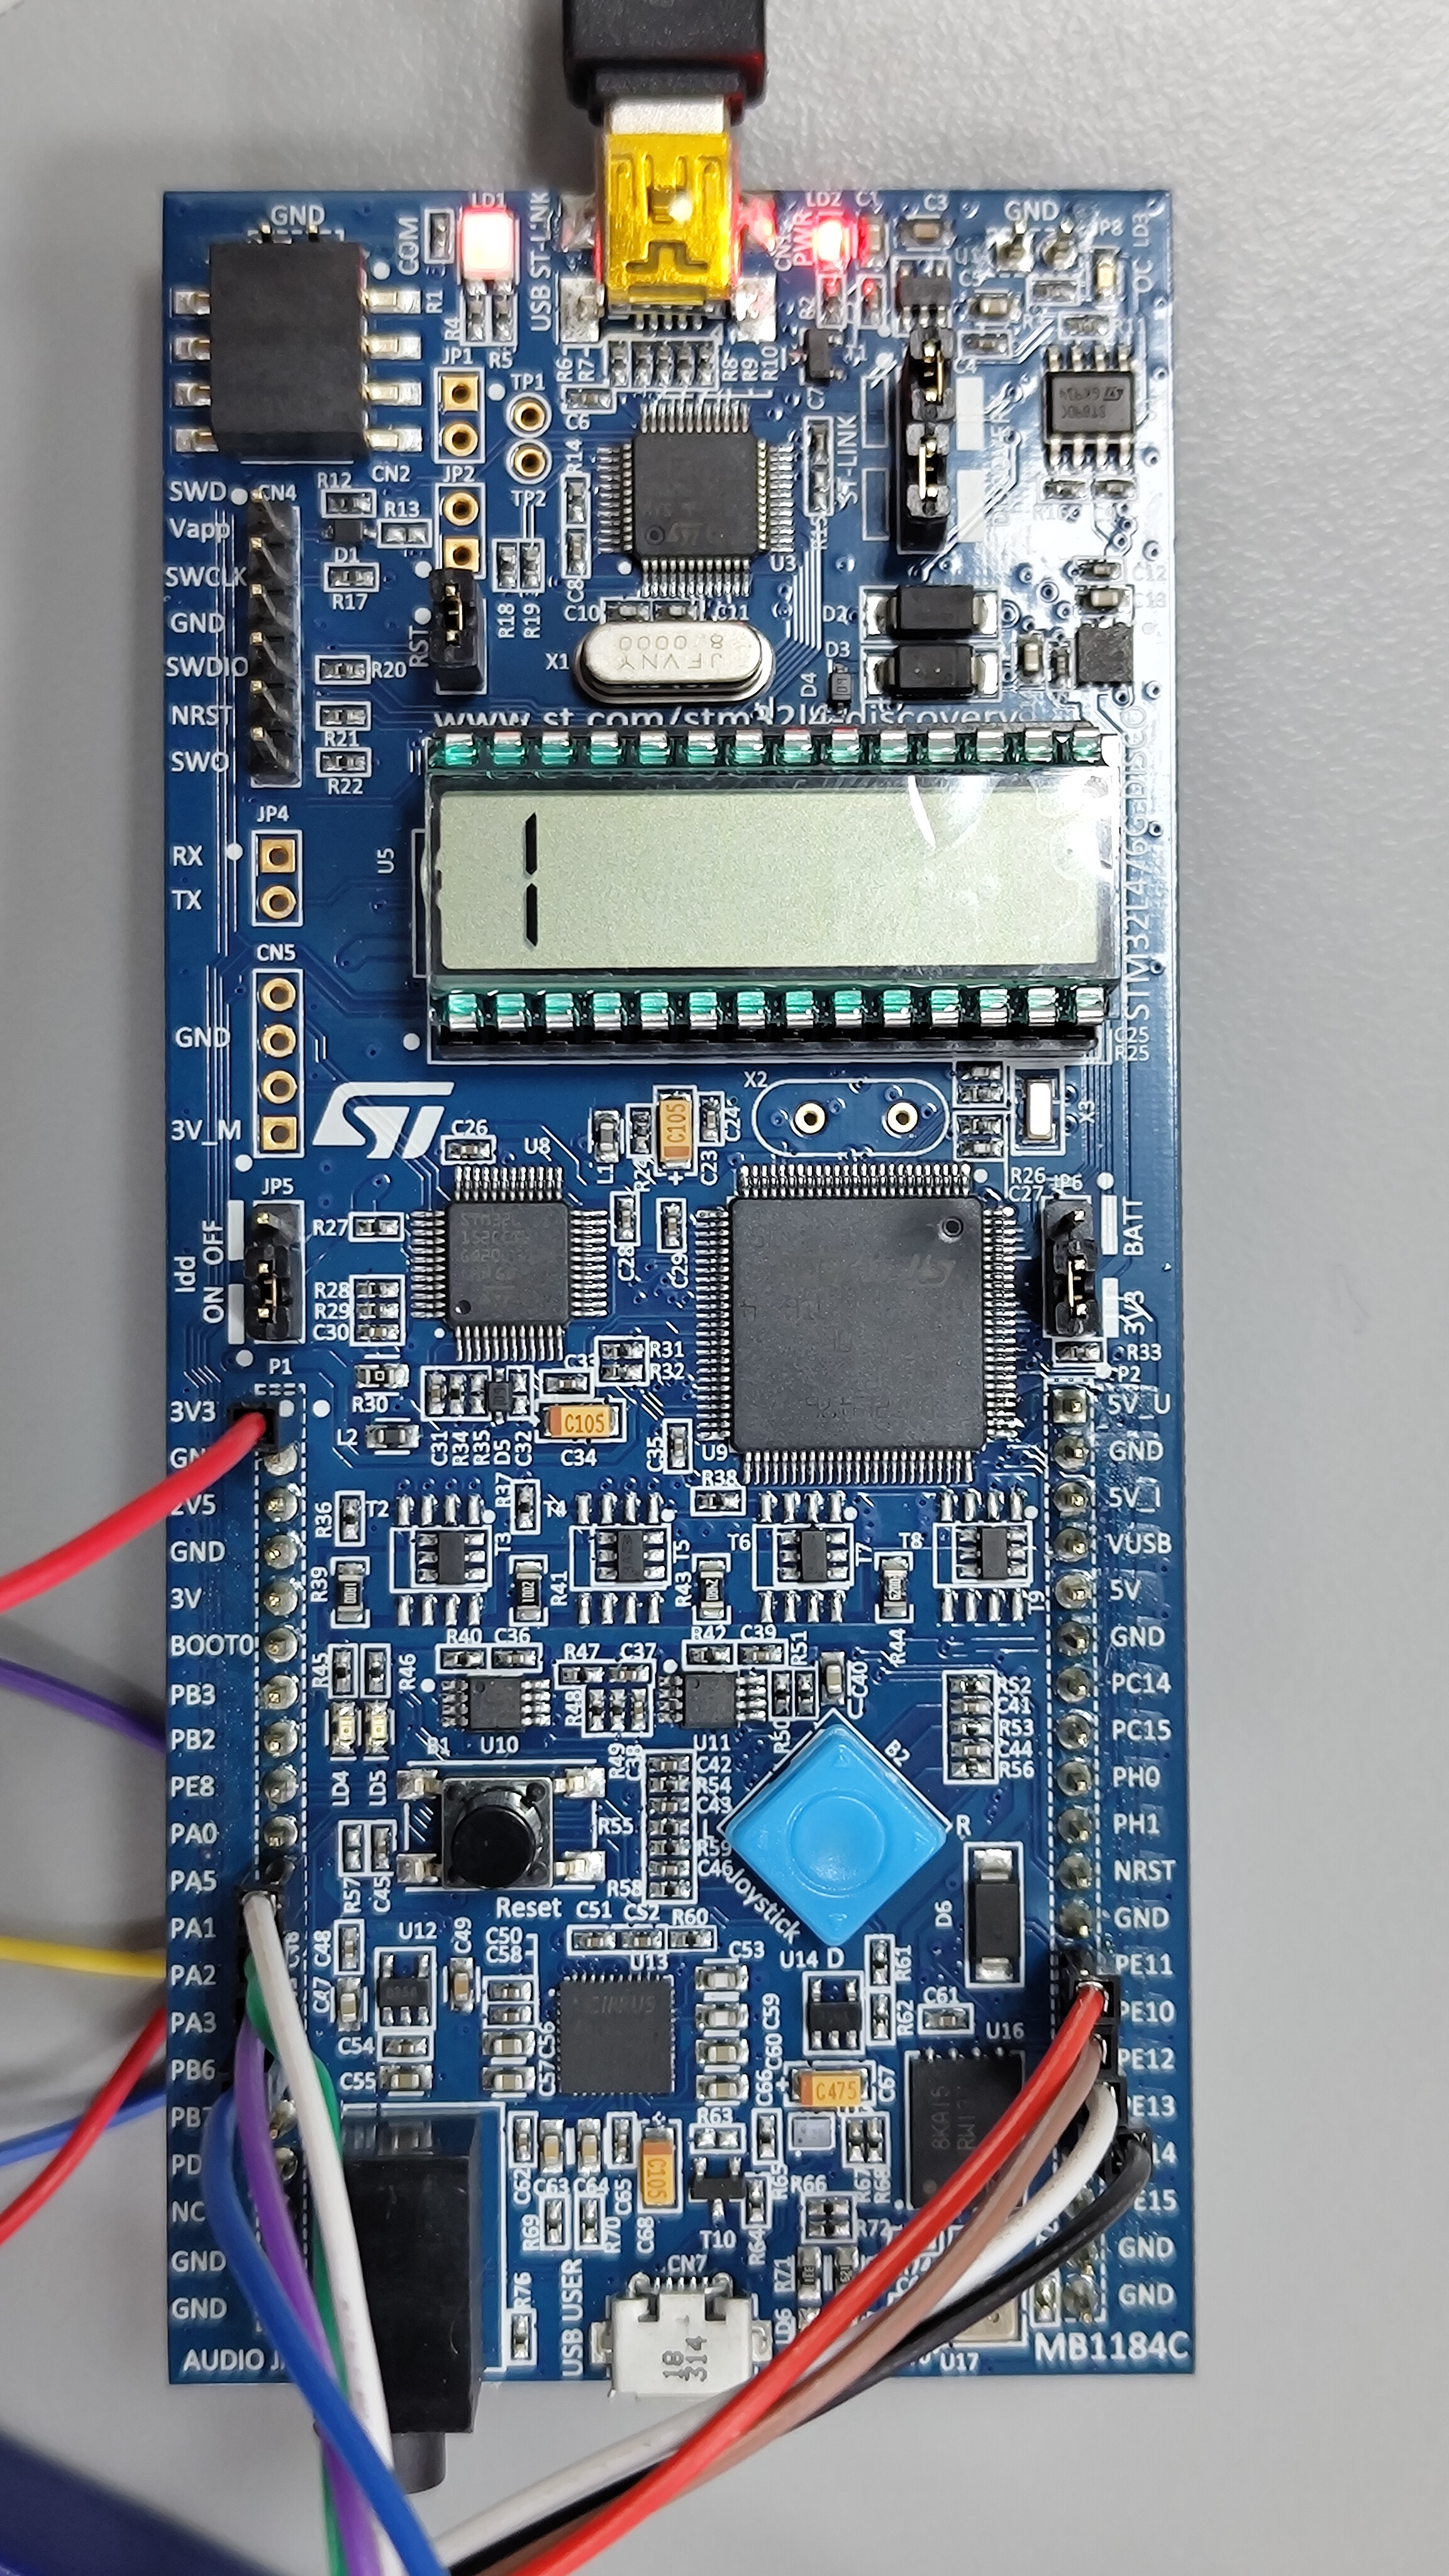
\includegraphics[width=\textwidth]{1.jpg}
    \caption{1}
    \end{minipage}
    \hfill
    \begin{minipage}{0.45\textwidth}
        \centering
    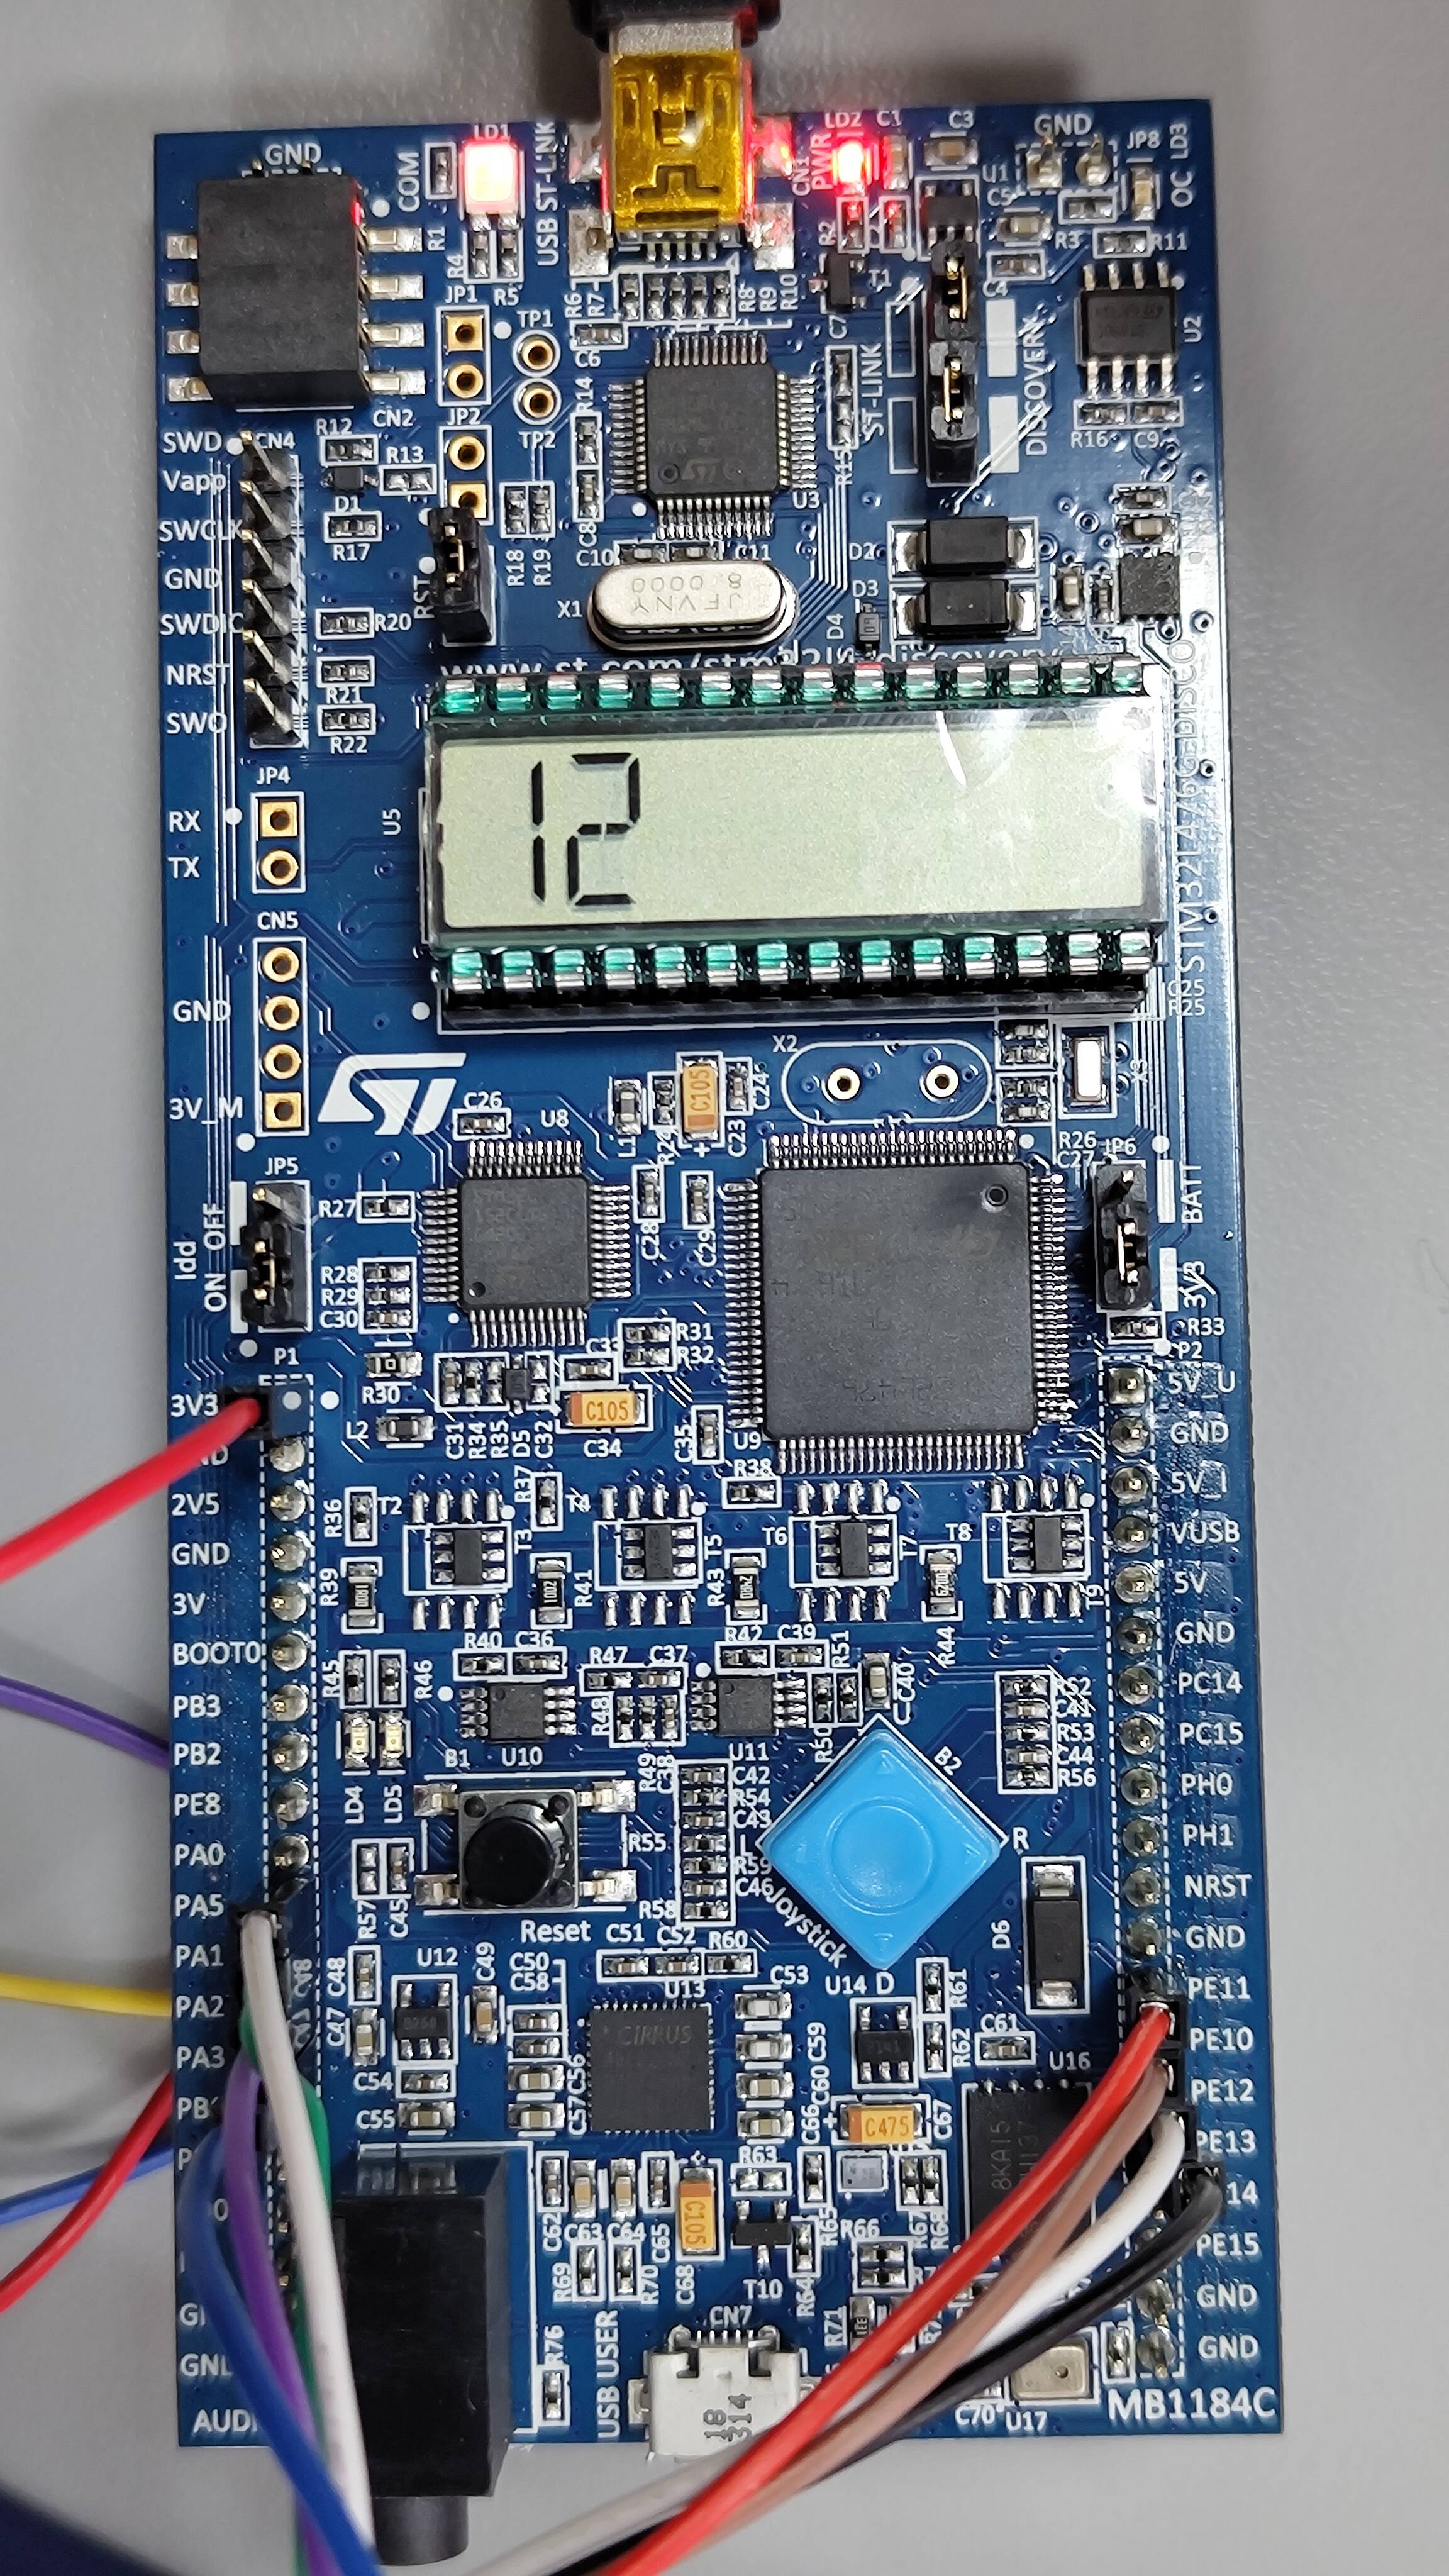
\includegraphics[width=\textwidth]{12.jpg}
    \caption{12}
\end{minipage}
    \hfill
    \end{figure}
\begin{figure}[h!]
    \centering
    \begin{minipage}{0.45\textwidth}
        \centering
    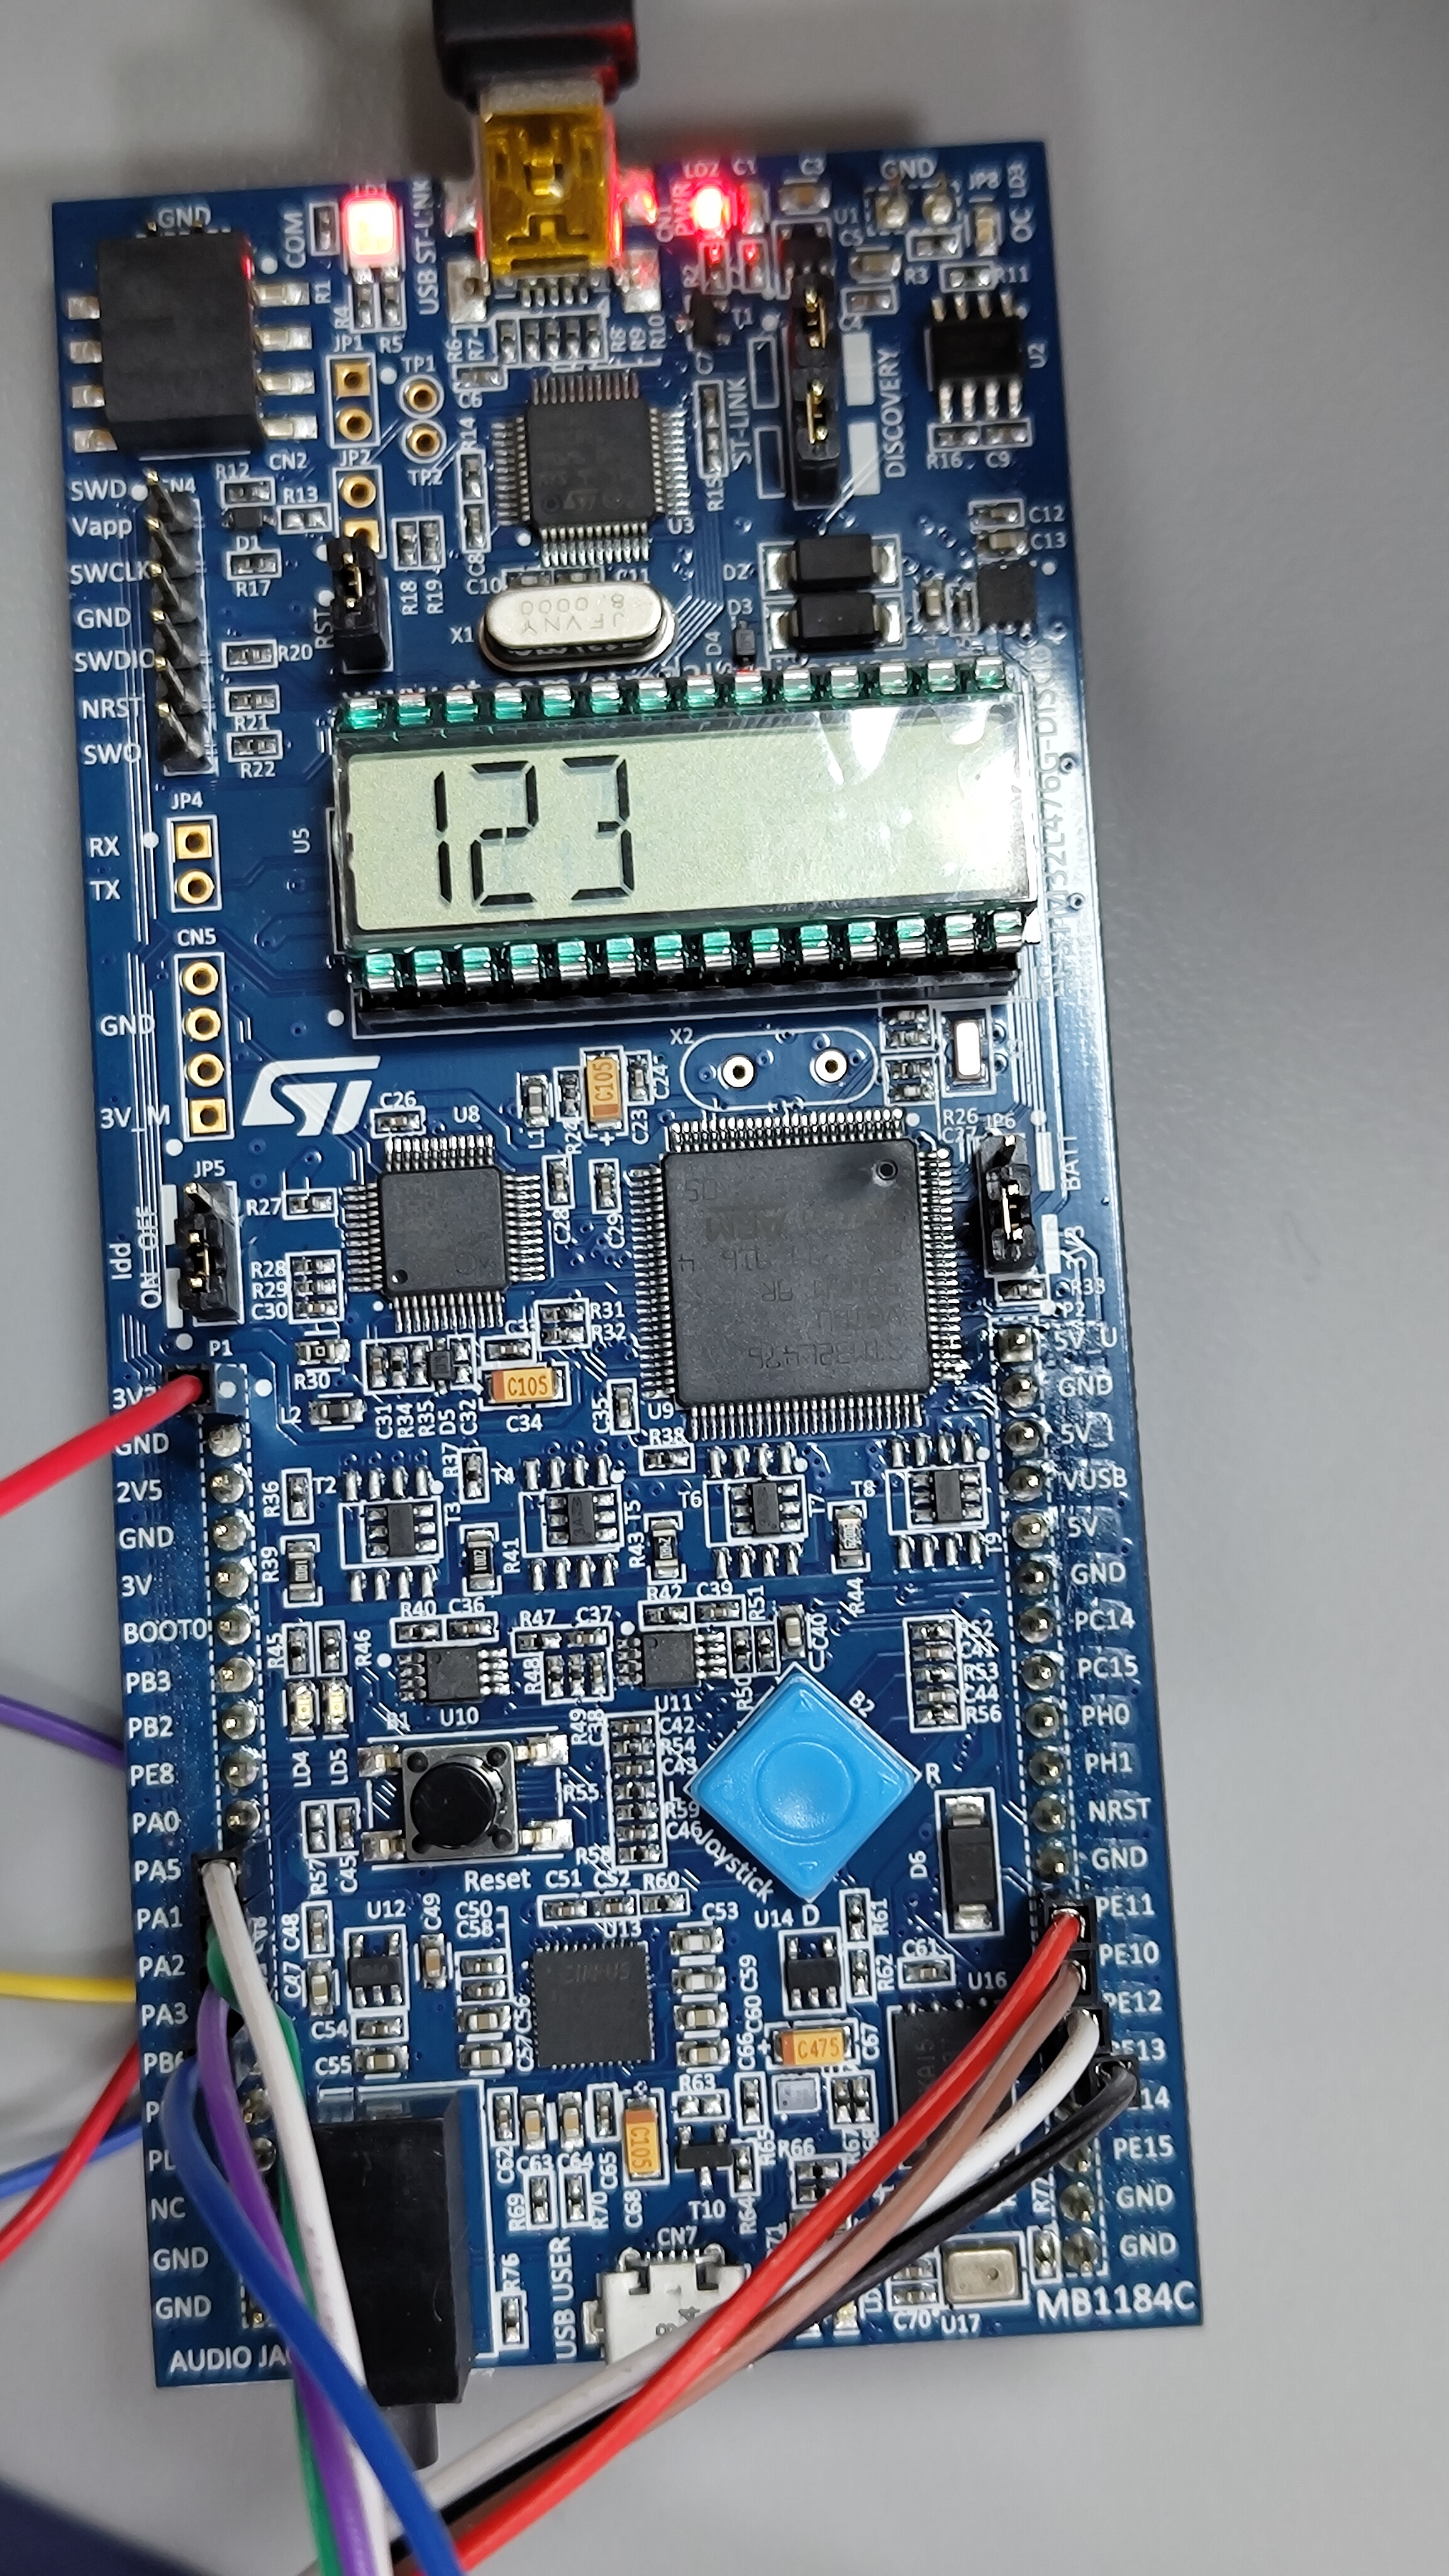
\includegraphics[width=\textwidth]{123.jpg}
    \caption{123}
\end{minipage}
    \hfill
    \begin{minipage}{0.45\textwidth}
        \centering
    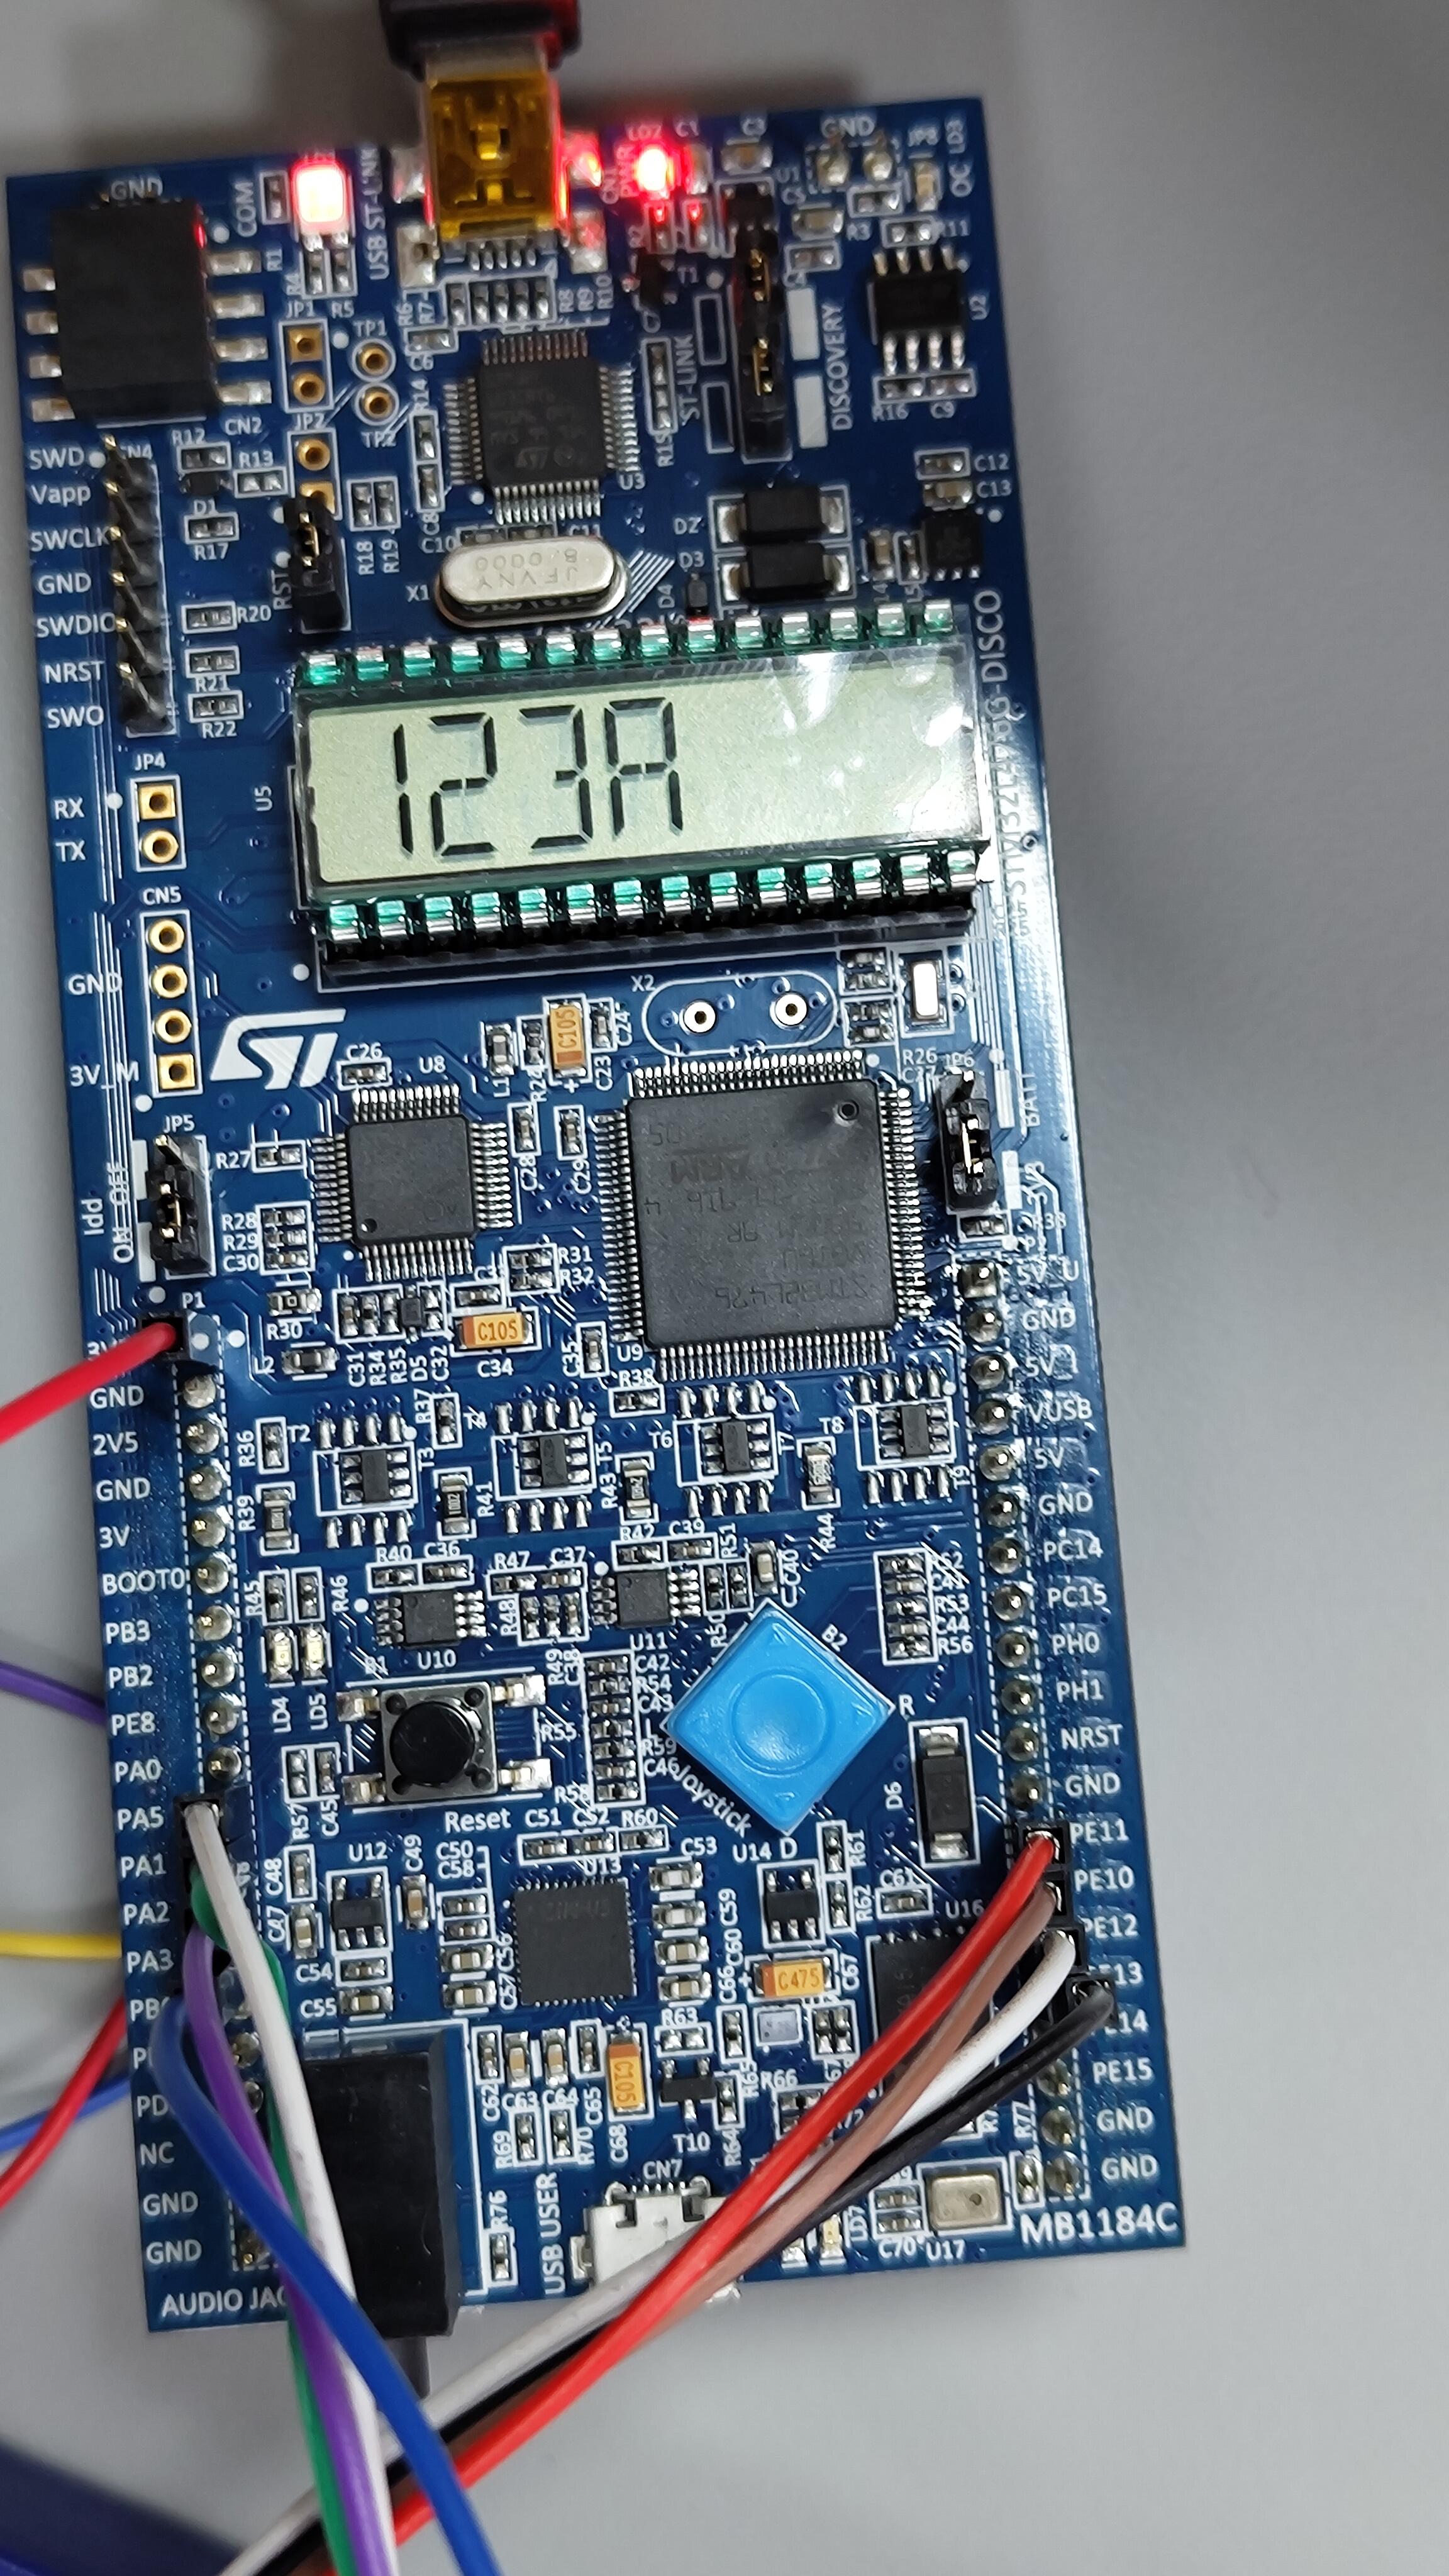
\includegraphics[width=\textwidth]{123A.jpg}
    \caption{123A}
    \end{minipage}
\end{figure}

\begin{figure}[H]
    \centering
    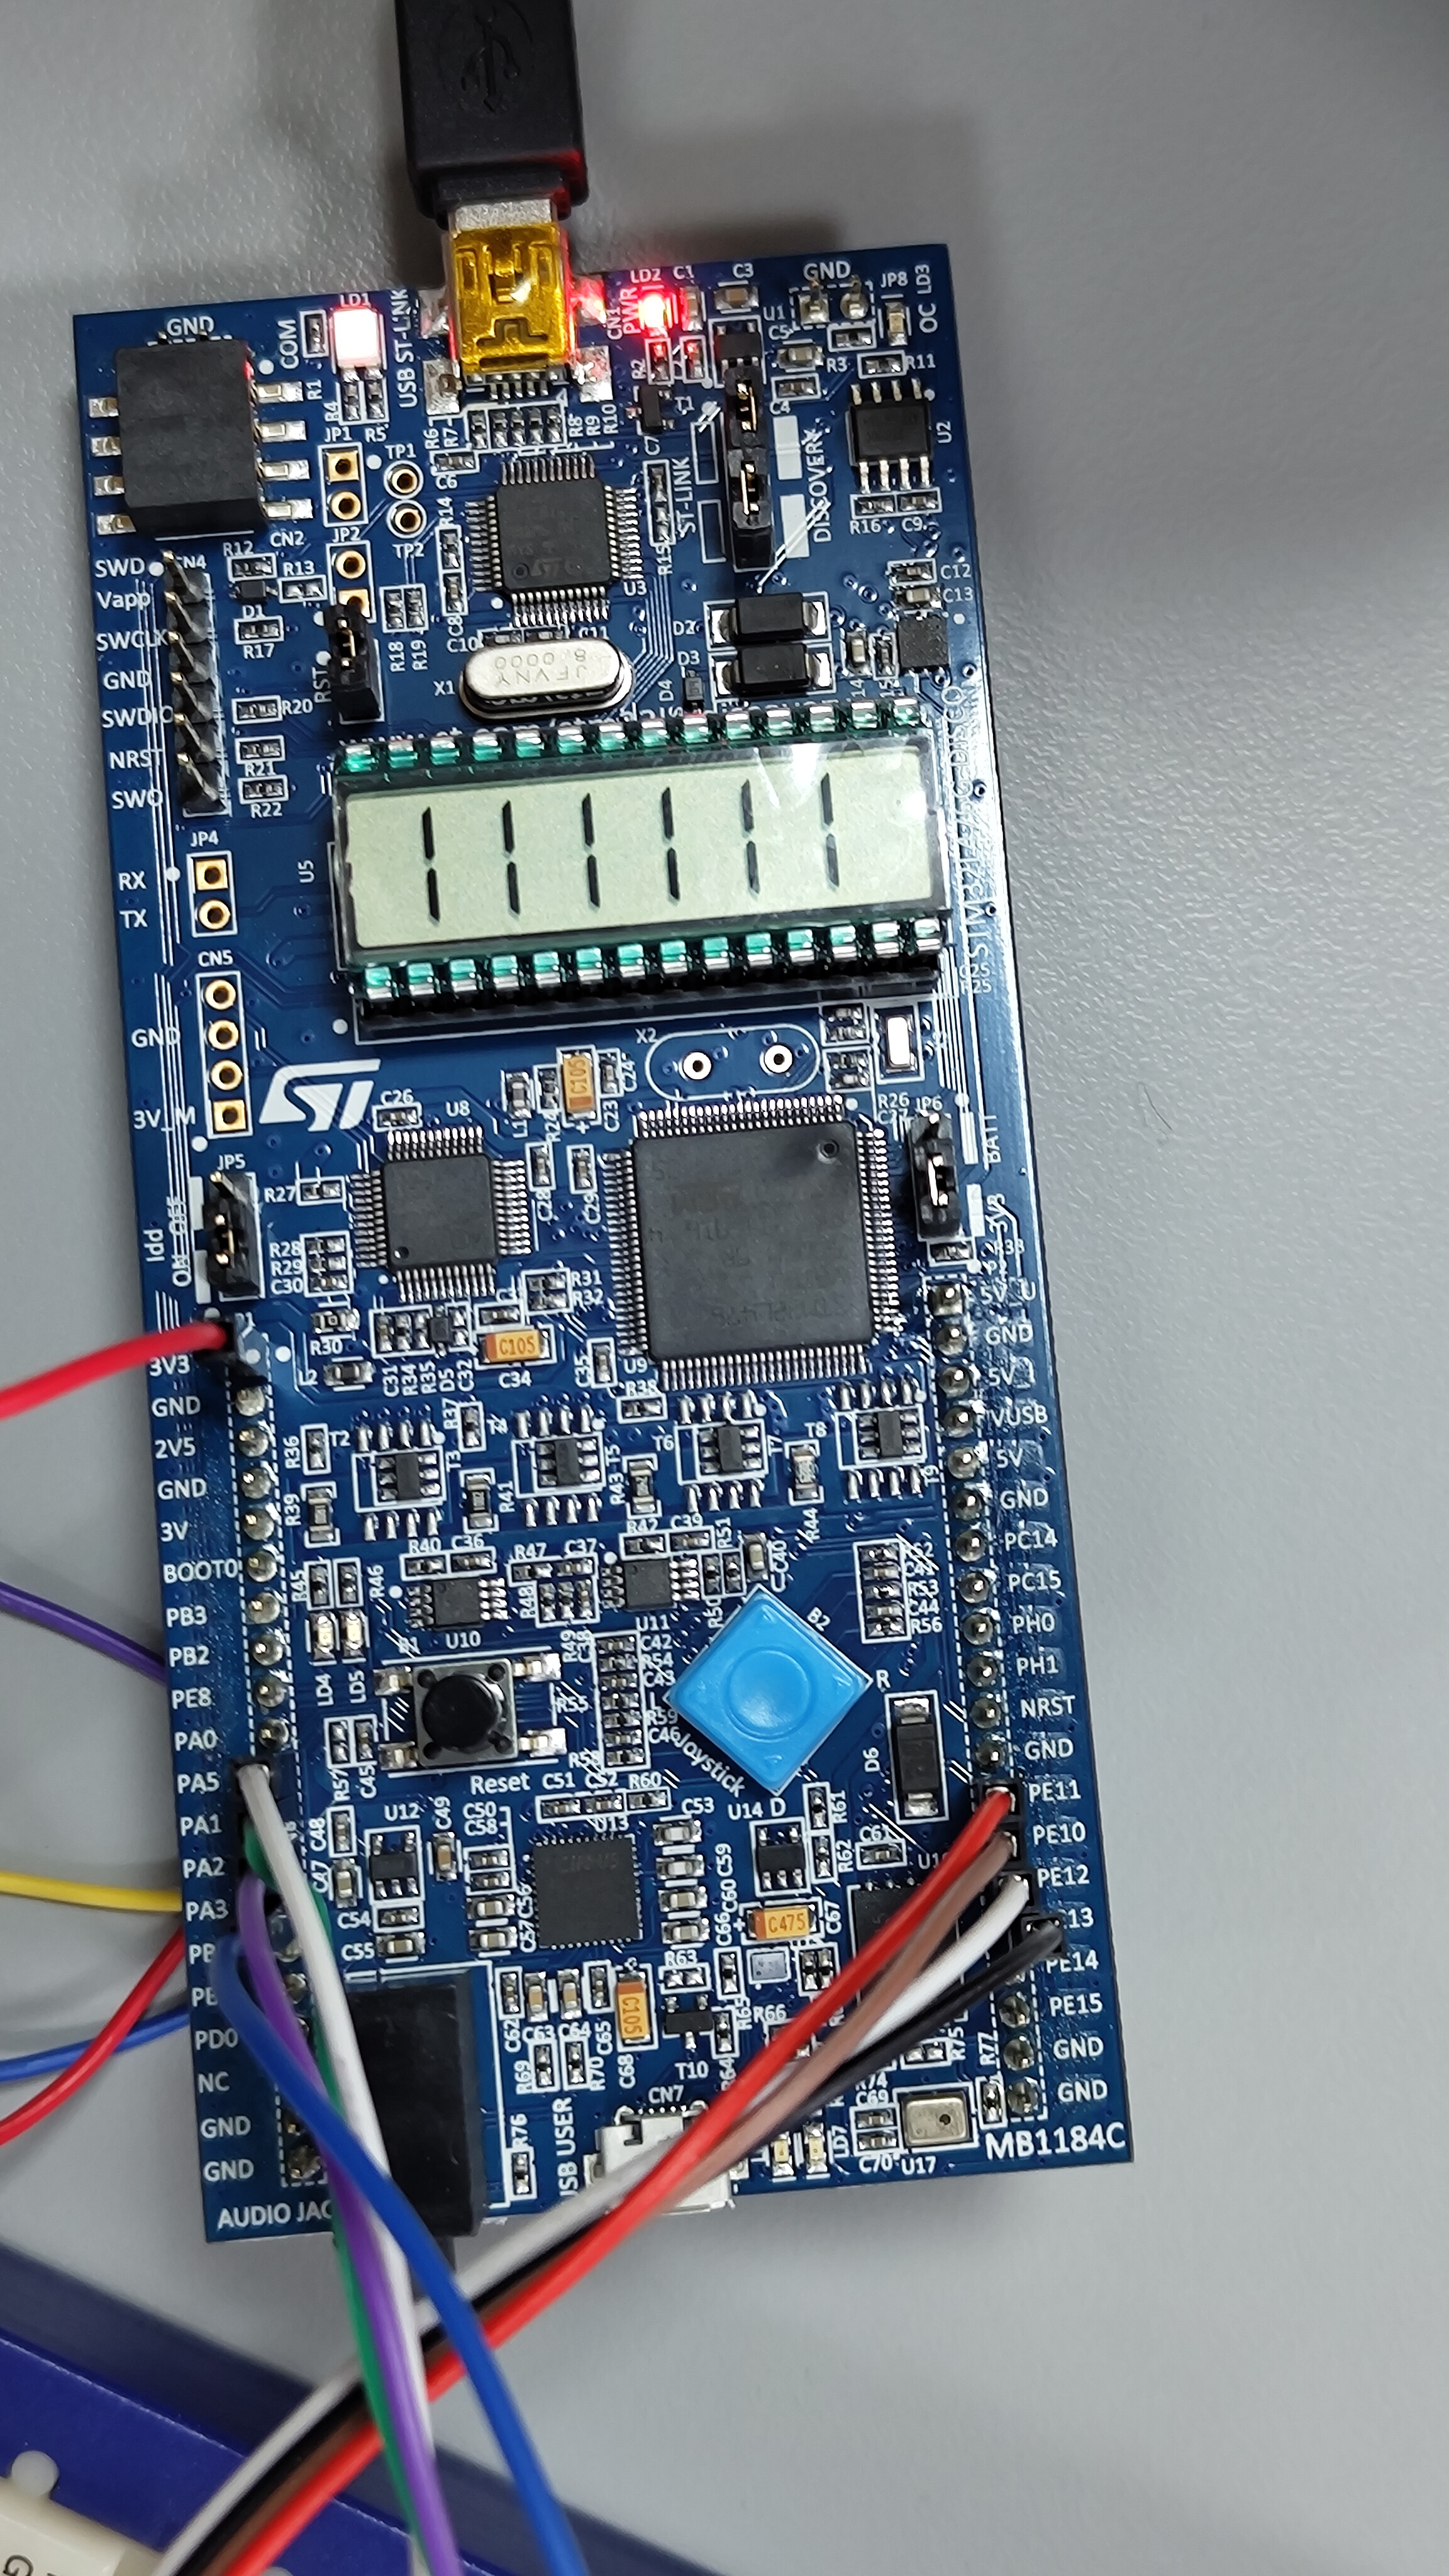
\includegraphics[width=0.4\textwidth]{1111.jpg}
    \caption{1111}
\end{figure}




\section{Code Implementation}

\subsection{Keypad Pin Initialization}
\begin{lstlisting}[language=C, caption={Keypad Pin Initialization}]
void Keypad_Pin_Init(void) {
    RCC->AHB2ENR |= RCC_AHB2ENR_GPIOAEN | RCC_AHB2ENR_GPIOEEN;

    GPIOE->MODER &= ~(3U<<(2*10) | 3U<<(2*11) | 3U<<(2*12) | 3U<<(2*13));
    GPIOE->MODER |=  (1U<<(2*10) | 1U<<(2*11) | 1U<<(2*12) | 1U<<(2*13));

    GPIOA->MODER &= ~(3U<<(2*1) | 3U<<(2*2) | 3U<<(2*3) | 3U<<(2*5));
}
\end{lstlisting}

\subsection{Keypad Scanning Function}
\begin{lstlisting}[language=C, caption={Keypad Scanning}]
char keypad_scan(void) {
    for (int row = 0; row < 4; row++) {
        GPIOE->ODR &= ~(0b1111 << 10);
        GPIOE->ODR |= ~(1 << (10 + row));
        delay(5);

        uint8_t col = (GPIOA->IDR >> 1) & 0b1011;

        if (col != 0xF) {
            for (int c = 0; c < 4; c++) {
                if (!(col & (1 << c))) {
                    return lookup[row][c]; 
                }
            }
        }
    }
    return 0xFF; 
}
\end{lstlisting}
\newpage
\subsection{LCD Display Update}
\begin{lstlisting}[language=C, caption={LCD Display Update}]
void update_lcd(char key) {
    for (int i = 0; i < 5; i++) {
        buffer[i] = buffer[i+1];
    }
    buffer[5] = key;
    LCD_DisplayString(buffer);
}
\end{lstlisting}

\section{C Program for LCD Configuration and Display}

The following C program configures and controls the LCD display in an STM32L476 microcontroller. It includes initialization functions, display control mechanisms, and character mapping for the LCD.

\begin{lstlisting}[language=C, caption={LCD Configuration and Display Code}, label={code:lcd_configuration}, basicstyle=\ttfamily\footnotesize, keywordstyle=\color{blue}, commentstyle=\color{gray}, stringstyle=\color{red}, breaklines=true, numbers=left, numberstyle=\tiny\color{gray}, frame=single]

#include "lcd.h"
#include "stm32l476xx.h"
#include <stdint.h>

/* =========================
         LCD MAPPING
   =========================
LCD allows displaying information on six 14-segment digits and 4 bars:

  1       2       3       4       5       6
-----   -----   -----   -----   -----   -----   
|\|/| o |\|/| o |\|/| o |\|/| o |\|/|   |\|/|   BAR3
-- --   -- --   -- --   -- --   -- --   -- --   BAR2
|/|\| o |/|\| o |/|\| o |/|\| o |/|\|   |/|\|   BAR1
----- * ----- * ----- * ----- * -----   -----   BAR0
*/

// Constant table for capital letters A to Z
const uint16_t CapLetterMap[26] = {
    0xFE00, 0x6714, 0x1d00, 0x4714, 0x9d00, 0x9c00, 0x3f00, 0xfa00, 0x0014,
    0x5300, 0x9841, 0x1900, 0x5a48, 0x5a09, 0x5f00, 0xFC00, 0x5F01, 0xFC01,
    0xAF00, 0x0414, 0x5b00, 0x18c0, 0x5a81, 0x00c9, 0x0058, 0x05c0
};

// Constant table for numbers 0 to 9
const uint16_t NumberMap[10] = {
    0x5F00, 0x4200, 0xF500, 0x6700, 0xEa00, 0xAF00, 0xBF00, 0x04600, 0xFF00, 0xEF00
};

// LCD Initialization
void LCD_PIN_Init(void) {
    // Enable GPIO clocks for PA, PB, PC, and PD
    RCC->AHB2ENR |= RCC_AHB2ENR_GPIOAEN | RCC_AHB2ENR_GPIOBEN | RCC_AHB2ENR_GPIOCEN | RCC_AHB2ENR_GPIODEN;

    // Configure GPIO mode as alternate function
    GPIOA->MODER &= 0x3FC00FFF;
    GPIOA->MODER |= 0x802AA000;

    GPIOB->MODER &= 0x00F3F0F0;
    GPIOB->MODER |= 0xAA080A0A;

    GPIOC->MODER &= 0xFFFC003F;
    GPIOC->MODER |= 0x0002AA80;

    GPIOD->MODER &= 0x0000FFFF;
    GPIOD->MODER |= 0xAAAA0000;

    // Configure Alternate Function Registers (AFR)
    GPIOA->AFR[0] &= 0x00FFFFFF;
    GPIOA->AFR[0] |= 0xBB000000;
    GPIOA->AFR[1] &= 0x0FFFF000;
    GPIOA->AFR[1] |= 0xB0000BBB;

    GPIOB->AFR[0] &= 0xFF00FF00;
    GPIOB->AFR[0] |= 0x00BB00BB;
    GPIOB->AFR[1] &= 0x0000FF0F;
    GPIOB->AFR[1] |= 0xBBBB00B0;

    GPIOC->AFR[0] &= 0x00000FFF;
    GPIOC->AFR[0] |= 0xBBBBB000;
    GPIOC->AFR[1] &= 0xFFFFFFF0;
    GPIOC->AFR[1] |= 0x0000000B;

    GPIOD->AFR[1] |= 0xBBBBBBBB;
}

// Function to display a string on the LCD
void LCD_DisplayString(uint8_t* ptr) {
    for (uint8_t i = 0; i < 6; i++) {
        LCD_WriteChar(ptr++, 0, 0, i);
    }
}

// Function to display a specific name on the LCD
void LCD_Display_Name(void) { 
    while ((LCD->SR & LCD_SR_UDR) != 0); // Wait for Update Display Request Bit

    // Display "SENERE"
    LCD->RAM[0] |= 0xD782A168;
    LCD->RAM[1] |= 0x00E; 
    LCD->RAM[2] |= 0xE5C25278; 
    LCD->RAM[3] |= 0x005; 
    LCD->RAM[6] |= 0x0000C000;
    LCD->RAM[7] |= 0x008; 

    LCD->SR |= LCD_SR_UDR; // Update LCD display
}

// LCD Configuration
void LCD_Configure(void) {
    LCD->CR &= ~LCD_CR_LCDEN;
    
    // Set bias to 1/3
    LCD->CR &= ~(0x03<<5);
    LCD->CR |= 0x02<<5;

    // Set duty to 1/4
    LCD->CR &= ~(0x07<<2); 
    LCD->CR |= 0x03<<2; 

    // Set contrast and pulse on period
    LCD->FCR |= LCD_FCR_CC | LCD_FCR_PON; 

    // Select internal voltage source
    LCD->CR &= ~LCD_CR_VSEL; 

    // Wait for LCD to be ready
    while ((LCD->SR & LCD_SR_FCRSR) == 0); 
    LCD->CR |= LCD_CR_LCDEN; 

    while ((LCD->SR & LCD_SR_ENS) == 0);
    while ((LCD->SR & LCD_SR_RDY) == 0);
}

// LCD Initialization Wrapper
void LCD_Initialization(void) {
    LCD_PIN_Init();
    LCD_Clock_Init();    
    LCD_Configure();
    LCD_Clear();
}

// LCD Clock Initialization
void LCD_Clock_Init(void) {
    RCC->APB1ENR1 |= RCC_APB1ENR1_PWREN;    
    if ((PWR->CR1 & PWR_CR1_DBP) == 0) {
        PWR->CR1 |= PWR_CR1_DBP;
        while((PWR->CR1 & PWR_CR1_DBP) == 0);
    }

    RCC->BDCR &= ~(RCC_BDCR_LSEON | RCC_BDCR_LSEBYP);
    RCC->BDCR |= RCC_BDCR_BDRST;
    RCC->BDCR &= ~RCC_BDCR_BDRST;

    while ((RCC->BDCR & RCC_BDCR_LSERDY) == 0) {
        RCC->BDCR |= RCC_BDCR_LSEON;
    }

    RCC->BDCR &= ~RCC_BDCR_RTCSEL;
    RCC->BDCR |= RCC_BDCR_RTCSEL_0;
    RCC->APB1ENR1 &= ~RCC_APB1ENR1_PWREN;
    RCC->APB1ENR1 |= RCC_APB1ENR1_LCDEN;
}

// Function to clear LCD display
void LCD_Clear(void) {
    while ((LCD->SR & LCD_SR_UDR) != 0);
    for (uint8_t counter = 0; counter <= 15; counter++) {
        LCD->RAM[counter] = 0;
    }
    LCD->SR |= LCD_SR_UDR;
}

\end{lstlisting}



\section{Post-Lab Questions}

\begin{enumerate}
    \item \textbf{Can your code correctly handle multiple keys pressed at once?}  
    \begin{itemize}
    \item \textbf{Answer:} No, the current approach detects only one key at a time. Handling multiple keypresses would require additional logic to track simultaneous key states.
\end{itemize}

    \item \textbf{How do you debounce keypresses?}  
    
    \begin{itemize}
    \item \textbf{Answer:} Debouncing is implemented by:
        \begin{itemize}
        \item Adding a small delay after detecting a keypress.
        \item Waiting for the key to be released before registering another press.
        \end{itemize}
    \end{itemize}

    \item \textbf{Why are external pull-up resistors used instead of internal ones?}  
    \begin{itemize}
        \item \textbf{Answer:} Internal pull-ups are around 40kohm, which is too weak for reliable operation. The 2.2kohm external pull-ups ensure proper voltage levels.
    \end{itemize}
    
\end{enumerate}

\section{Conclusion}

This lab successfully demonstrated the implementation of a keypad scanning system using the STM32L476G-DISCO microcontroller, integrating hardware and software techniques to detect and display keypresses dynamically on an LCD screen. The experiment provided hands-on experience in configuring GPIO pins for input and output, utilizing pull-up resistors, and implementing a software debouncing mechanism to ensure reliable key detection.

Key takeaways from this lab include:
\begin{itemize}
    \item Understanding the principles of matrix keypad interfacing and GPIO configuration for effective row-column scanning.
    \item Developing a real-time keypad scanning algorithm that efficiently detects keypresses and prevents ghosting effects.
    \item Implementing software debouncing techniques to eliminate false triggers and ensure accurate input recognition.
    \item Designing a dynamic LCD update mechanism that allows for smooth scrolling of keypresses, emulating behavior found in calculators and electronic keypads.
\end{itemize}

The results of this lab demonstrate the effectiveness of embedded system programming in handling human-machine interfaces (HMI) and real-time interactions. The successful integration of the keypad and LCD display paves the way for more complex applications, such as password-protected access systems, interactive menu navigation, and embedded UI development.

Future improvements could include multi-keypress detection, interrupt-based scanning, and event-driven input processing, enhancing the system’s efficiency and responsiveness. This lab has provided a strong foundation for implementing real-world embedded applications that rely on efficient input handling and user interaction.

\end{document}


\end{document}
